\documentclass[a4paper, 10pt]{article}
\usepackage[english]{babel}
\usepackage[utf8]{inputenc}
\usepackage{enumitem}
\usepackage{float}
\usepackage{titlesec}
\usepackage{framed}
\usepackage{listings}
\usepackage{graphicx}
\usepackage{titling}
\usepackage{blindtext}
\usepackage{amsmath}  % for \hookrightarrow
\usepackage{xcolor}   % for \textcolor
\graphicspath{ {../ER/} }
\usepackage[hmargin=2cm,vmargin=3.5cm,bmargin=2cm]{geometry}

\setlist[itemize]{noitemsep, topsep=0pt}
\setlength\parindent{0pt}

\setcounter{secnumdepth}{0} %% no numbering

\begin{document}
\title{Advanced DataBases C4 Group\\\
  \huge Bank Management System}
\author{
  Samuel Lúcio Vicente, 251720
  \and
  Daniel Silva, 251702
  \and
  Jorge Marrero Camiruaga, 251438
}

\date{Politechnika Wrocławska\\today}

\maketitle

\lstset{
  basicstyle=\small\ttfamily,
  frame=lrtb,
  numbers=left,
  columns=fullflexible,
  breaklines=true,
  postbreak=\mbox{\textcolor{red}{$\hookrightarrow$}\space}
}

\section{Improvements}

\subsection{Query 1}
\subsubsection{SQL}
\begin{lstlisting}[language=SQL]
UPDATE Account 
SET amount = amount*2 
WHERE amount <= ALL(
        SELECT Avg(amount) 
        FROM Account 
);

SELECT Name
    FROM Costumer
    INNER JOIN Person
        ON GovID = PersonGovID 
    INNER JOIN Account 
        ON CostumerID = CostumerCostumerID
    WHERE amount >= ALL(
        SELECT MAX(amount) 
        FROM Account 
);
\end{lstlisting}

\subsection{First Improvement}
\begin{itemize}
  \item B-Tree index on Account based on the amount
\end{itemize}
\subsubsection{Times}
\begin{table}[H]
\begin{tabular}{l|l|l|l|l|}
\cline{2-5}
\textbf{}                             & \textbf{Max} & \textbf{Min} & \textbf{Avg} & \textbf{\#}  \\ \hline
\multicolumn{1}{|l|}{\textbf{Before}} & 3,49          & 2,88          & 3,086          & 5            \\ \hline
\multicolumn{1}{|l|}{\textbf{After}}  & 4,98          & 4,56          & 4,788          & 5            \\ \hline
\end{tabular}
\end{table}
\subsubsection{Observations}
Longer times with the INDEX enabled.\\ 
This might seem counterintuitive has now in the UPDATE statement we see that instead of a TABLE ACCESS FULL we see a INDEX RANGE SCAN, which should be faster since less rows are being fetched, although thats true when using a INDEX in UPDATE statements and in our case updating the column on which the INDEX is based on brings with it more memory accesses and CPU time to keep the INDEX upto date with the changes being made. If we check the stats for this execution with and without the INDEX we see that there is a lot more physical read total IO requests for when the INDEX is in use, 46 vs 225 when not in use.\\ 
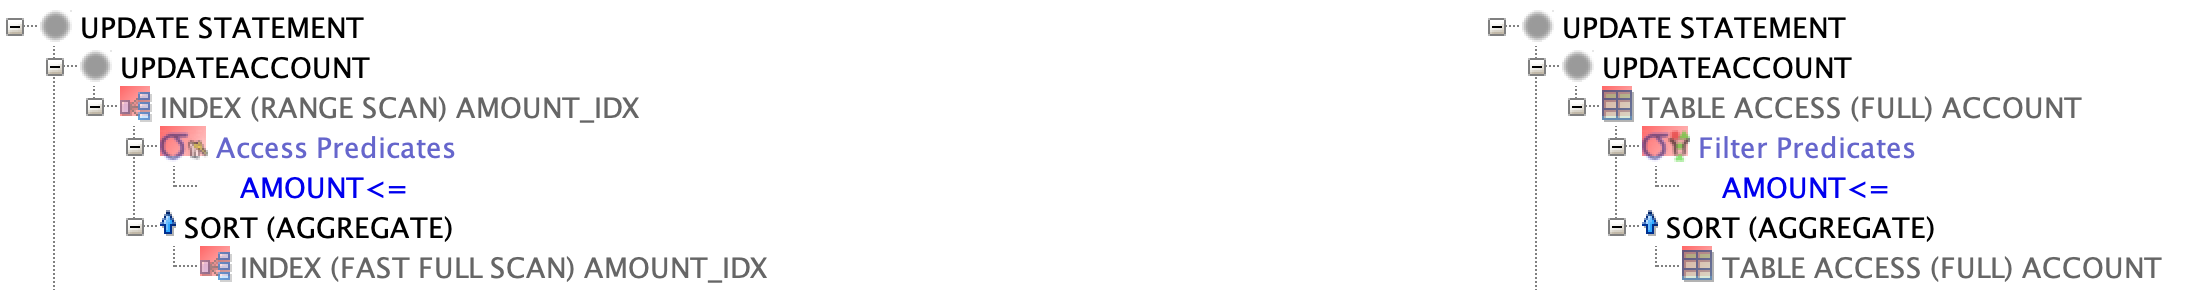
\includegraphics[width=\textwidth,height=\textheight,keepaspectratio]{1UPDATE}\\ 
The SELECT statement gets better with the index, as it should since there is now a INDEX RANGE SCAN instead of a TABLE ACCESS FULL when joining the Account table. We see that in the stats the physical read total IO requests for when the INDEX is in use is 8 vs 14 when not in use, we also see that in the session logical reads we have much more accesses to the memory per second 892 vs 216 when the index is in use.\\
\includegraphics[width=\textwidth,height=\textheight,keepaspectratio]{1selectCompare}\\
Although we see that the SELECT statement got better with the INDEX its improvements aren't enough to cover the performance hit the UPDATE query got.\\
\subsection{Second Improvement}
\begin{itemize}
  \item Partition Account by range of amount
\end{itemize}

\subsubsection{Times}
\begin{table}[H]
\begin{tabular}{l|l|l|l|l|}
\cline{2-5}
\textbf{}                             & \textbf{Max} & \textbf{Min} & \textbf{Avg} & \textbf{\#}  \\ \hline
\multicolumn{1}{|l|}{\textbf{Before}} & 3,49          & 2,88          & 3,086          & 5            \\ \hline
\multicolumn{1}{|l|}{\textbf{After}}  & 18,6         & 13,73         & 15,202          & 5            \\ \hline
\end{tabular}
\end{table}
\subsubsection{Observations}
Again longer times with partition.\\
We see that there is Partition pruning but since we are updating the column that the partition is based on then it has to move the new values to their new partitions which takes time and negates the effort of partitioning the tables.\\
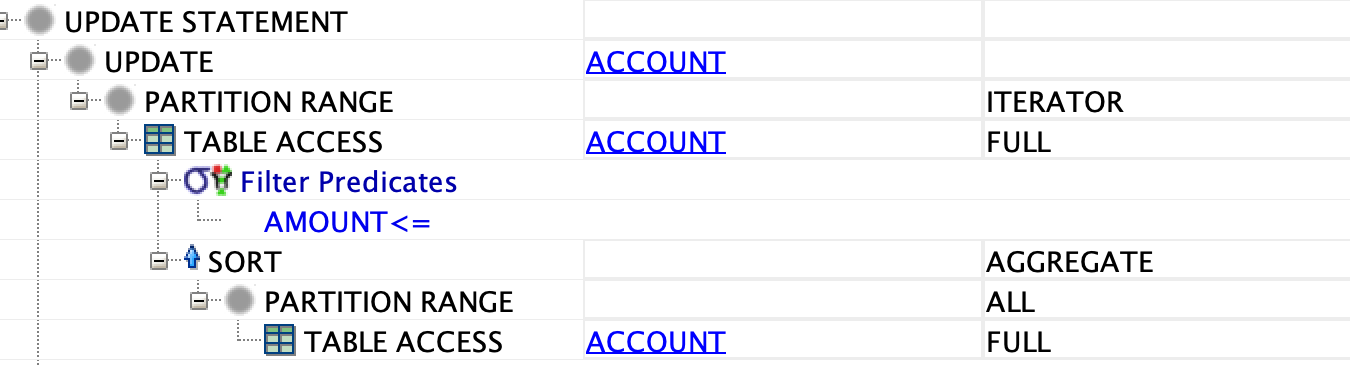
\includegraphics[width=\textwidth,height=\textheight,keepaspectratio]{2update}\\ 
The SELECT statement gets better with the partition, as it should since there is now a PARTITION RANGE ITERATOR instead of a TABLE ACCESS FULL when joining the Account table. We see that in the stats the physical read total IO requests for when the PARTITION is in use is 0 vs 14 when not in use, we also see that in the session logical reads we have much more accesses to the memory per second 892 vs 617 when the PARTITION is in use.\\
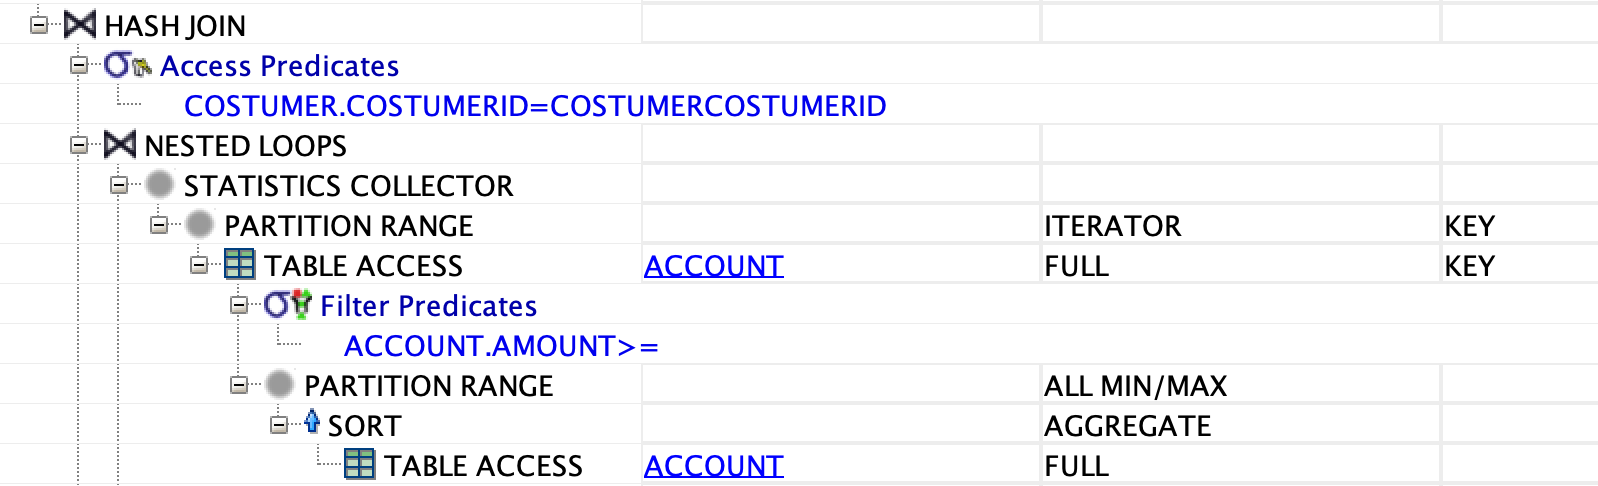
\includegraphics[width=\textwidth,height=\textheight,keepaspectratio]{2Select}\\
From this we can conclude that using an INDEX or a PARTITION based on the column we are updating is a bad practice since it forces the INDEX/PARTITION to rearrange to keep track of changes which is very expensive. From this we can gather also that keeping PARTITIONs upto date is much more expensive than keeping INDEXs upto date.\\

\subsection{Query 2}
\subsubsection{SQL}
\begin{lstlisting}[language=SQL]
ALTER SYSTEM FLUSH BUFFER_CACHE;
ALTER SYSTEM FLUSH SHARED_POOL;

SET TIMING ON;
select count(*)
from savingsaccount inner join Account
    on AccountAccountID = AccountID
inner join Costumer
    on CostumerCostumerID = CostumerID
inner join Person
    on PersonGovID = GovID
where durationyears>7 and Nationality = 'Poland';

update SavingsAccount
set interestRate =
CASE
    WHEN durationYears>7 THEN interestrate + 0.03
    ELSE interestrate + 0.01
END;
\end{lstlisting}

\subsection{Third Improvement}
\begin{itemize}
  \item List partition in Person based on the nationalities
  \item Range partition in SavingsAccount based on duration years, one partition for values bigger than 7 and one for smaller than
\end{itemize}
\subsubsection{Times}
\begin{table}[H]
\begin{tabular}{l|l|l|l|l|}
\cline{2-5}
\textbf{}                             & \textbf{Max} & \textbf{Min} & \textbf{Avg} & \textbf{\#}  \\ \hline
\multicolumn{1}{|l|}{\textbf{Before}} & lol         & lol         & lol          & 5            \\ \hline
\multicolumn{1}{|l|}{\textbf{After}}  & lol         & lol         & lol          & 5            \\ \hline
\end{tabular}
\end{table}
\subsubsection{Observations}
lol
\includegraphics[width=\textwidth,height=\textheight,keepaspectratio]{lol}\\ 
lol
\includegraphics[width=\textwidth,height=\textheight,keepaspectratio]{lol}\\
lol

\subsection{Query 3}
\subsubsection{SQL}
\begin{lstlisting}[language=SQL]
DECLARE 
    costID NUMBER:=1;
    
BEGIN

WHILE costID<700
LOOP
  UPDATE Account 
SET amount =     
  CASE          
      WHEN (
      SELECT EXTRACT(YEAR FROM CURRENT_DATE) - EXTRACT(YEAR FROM (
          SELECT BeginDate 
          FROM Account INNER JOIN SavingsAccount 
            ON AccountID=AccountAccountID 
          WHERE AccountAccountID=(
            select min(AccountID) 
            from Account inner join SavingsAccount 
                on AccountAccountID=AccountID 
            where CostumerCostumerID=costID)))
        AS year FROM dual) > (
          SELECT DurationYears 
          FROM SavingsAccount 
          WHERE AccountAccountID=(
            select min(AccountID) 
            from Account inner join SavingsAccount 
                on AccountAccountID=AccountID 
            where CostumerCostumerID=costID))
      THEN amount + ( 
          SELECT (amount+1)*12*DurationYears*InterestRate 
          FROM  SavingsAccount INNER JOIN Account 
          ON AccountID=AccountAccountID 
          WHERE AccountAccountID=(
            select min(AccountID) 
            from Account inner join SavingsAccount 
                on AccountAccountID=AccountID 
            where CostumerCostumerID=costID))   
      ELSE amount + ( 
      SELECT amount 
      FROM  SavingsAccount INNER JOIN Account 
      ON AccountID=AccountAccountID 
      WHERE AccountAccountID=(
            select min(AccountID) 
            from Account inner join SavingsAccount 
                on AccountAccountID=AccountID 
            where CostumerCostumerID=costID)) 
  END 
WHERE AccountID = (
    SELECT AccountID 
    FROM CurrentAccount INNER JOIN Account 
        ON AccountID=AccountAccountID 
    WHERE AccountAccountID=(
            select min(AccountID) 
            from Account inner join CurrentAccount 
                on AccountAccountID=AccountID 
            where CostumerCostumerID=costID));

INSERT INTO Transfer(TransferDate, Amount, AccountAccountIDFrom, AccountAccountIDTo) VALUES (CURRENT_DATE, (
Select
  CASE
      WHEN (
          SELECT EXTRACT(YEAR FROM CURRENT_DATE) - EXTRACT(YEAR FROM (
              SELECT BeginDate 
              FROM Account INNER JOIN SavingsAccount 
                ON AccountID=AccountAccountID WHERE AccountAccountID=(
            select min(AccountID) 
            from Account inner join SavingsAccount 
                on AccountAccountID=AccountID 
            where CostumerCostumerID=costID))) 
          AS year FROM dual) > (
              SELECT DurationYears 
              FROM SavingsAccount 
              WHERE AccountAccountID=(
            select min(AccountID) 
            from Account inner join SavingsAccount 
                on AccountAccountID=AccountID 
            where CostumerCostumerID=costID))
      THEN  amount*12*DurationYears*InterestRate
      ELSE  amount
  END
FROM SavingsAccount INNER JOIN Account
        ON AccountID=AccountAccountID
    WHERE AccountAccountID=(
            select min(AccountID) 
            from Account inner join SavingsAccount 
                on AccountAccountID=AccountID 
            where CostumerCostumerID=costID)),(
            select min(AccountID) 
            from Account inner join SavingsAccount 
                on AccountAccountID=AccountID 
            where CostumerCostumerID=costID), (
            select min(AccountID) 
            from Account inner join CurrentAccount 
                on AccountAccountID=AccountID 
            where CostumerCostumerID=costID));

UPDATE Account
SET amount = 0
WHERE AccountID = (
    SELECT AccountID 
    FROM SavingsAccount INNER JOIN Account 
        ON AccountID=AccountAccountID 
    WHERE AccountAccountID=(
            select min(AccountID) 
            from Account inner join SavingsAccount 
                on AccountAccountID=AccountID 
            where CostumerCostumerID=costID));
costID:=costID+1;
END LOOP;
END;
\end{lstlisting}

\subsection{Fourth Improvement}
\begin{itemize}
  \item Allocate SavingAccount and CurrentAccount in same disk and Account in another disk
\end{itemize}
\subsubsection{Times}
\begin{table}[H]
\begin{tabular}{l|l|l|l|l|}
\cline{2-5}
\textbf{}                             & \textbf{Max} & \textbf{Min} & \textbf{Avg} & \textbf{\#}  \\ \hline
\multicolumn{1}{|l|}{\textbf{Before}} & lol         & lol         & lol          & 5            \\ \hline
\multicolumn{1}{|l|}{\textbf{After}}  & lol         & lol         & lol          & 5            \\ \hline
\end{tabular}
\end{table}
\subsubsection{Observations}
lol
\includegraphics[width=\textwidth,height=\textheight,keepaspectratio]{lol}\\ 
lol
\includegraphics[width=\textwidth,height=\textheight,keepaspectratio]{lol}\\
lol

\subsection{Query 4}
\subsubsection{SQL}
\begin{lstlisting}[language=SQL]
DECLARE 
    empID NUMBER := 1;

BEGIN
WHILE empID<5000
LOOP
    INSERT INTO RoleHistory(RoleRoleID, EmployeeEmployeeID, BranchBranchId, BeginDate, EndDate) VALUES (
    1,
    empID,
    (SELECT BranchBranchID FROM RoleHistory WHERE EmployeeEmployeeID = empID AND EndDate is NULL),
    CURRENT_DATE,
    NULL);

    UPDATE RoleHistory
        SET EndDate = CURRENT_DATE
    WHERE HistoryID = (SELECT min(HistoryID) FROM RoleHistory WHERE EmployeeEmployeeID = empID AND EndDate is NULL);

empID:=empID+1;
END LOOP;
END;
\end{lstlisting}

\subsection{Fifth Improvement}
\begin{itemize}
  \item Hash partition RoleHistory by EmployeeEmployeeID and separate them in diferent disks
\end{itemize}
\subsubsection{Times}
\begin{table}[H]
\begin{tabular}{l|l|l|l|l|}
\cline{2-5}
\textbf{}                             & \textbf{Max} & \textbf{Min} & \textbf{Avg} & \textbf{\#}  \\ \hline
\multicolumn{1}{|l|}{\textbf{Before}} & lol         & lol         & lol          & 5            \\ \hline
\multicolumn{1}{|l|}{\textbf{After}}  & lol         & lol         & lol          & 5            \\ \hline
\end{tabular}
\end{table}
\subsubsection{Observations}
lol
\includegraphics[width=\textwidth,height=\textheight,keepaspectratio]{lol}\\ 
lol
\includegraphics[width=\textwidth,height=\textheight,keepaspectratio]{lol}\\
lol

\subsection{Sixth Improvement}
\begin{itemize}
  \item BitMap index in RoleHistory based in EndDate of RoleHistory if null or not
\end{itemize}
\subsubsection{Times}
\begin{table}[H]
\begin{tabular}{l|l|l|l|l|}
\cline{2-5}
\textbf{}                             & \textbf{Max} & \textbf{Min} & \textbf{Avg} & \textbf{\#}  \\ \hline
\multicolumn{1}{|l|}{\textbf{Before}} & lol         & lol         & lol          & 5            \\ \hline
\multicolumn{1}{|l|}{\textbf{After}}  & lol         & lol         & lol          & 5            \\ \hline
\end{tabular}
\end{table}
\subsubsection{Observations}
lol
\includegraphics[width=\textwidth,height=\textheight,keepaspectratio]{lol}\\ 
lol
\includegraphics[width=\textwidth,height=\textheight,keepaspectratio]{lol}\\
lol

\subsection{Seventh Improvement}
\begin{itemize}
  \item List partition in RoleHistory based on the EndDate being null or not
  \item B-Tree index based on the EmployeeEmployeeID
\end{itemize}
\subsubsection{Times}
\begin{table}[H]
\begin{tabular}{l|l|l|l|l|}
\cline{2-5}
\textbf{}                             & \textbf{Max} & \textbf{Min} & \textbf{Avg} & \textbf{\#}  \\ \hline
\multicolumn{1}{|l|}{\textbf{Before}} & lol         & lol         & lol          & 5            \\ \hline
\multicolumn{1}{|l|}{\textbf{After}}  & lol         & lol         & lol          & 5            \\ \hline
\end{tabular}
\end{table}
\subsubsection{Observations}
lol
\includegraphics[width=\textwidth,height=\textheight,keepaspectratio]{lol}\\ 
lol
\includegraphics[width=\textwidth,height=\textheight,keepaspectratio]{lol}\\
lol
\end{document}
